\chapter{Multiscale Score Matching}
\label{ch:msma}

This chapter will introduce Multiscale Score Matching Analysis (MSMA); my method for outlier detection via score norms. The first sections will explore the intuition behind score-norms and the need for multiple scales. The latter sections empirically demonstrate MSMA's best-in-class performance on OOD benchmarks. Note that this work used Noise Conditioned Score Networks (NCSNs)~\cite{Song2019}, which have been superseded by diffusion models (employed in later chapters). However, NCSNs laid the foundation and proof of concept upon which the rest of the research was developed.

\section{Multiscale Score Analysis}
\label{multiscale}
Recall that a score is the gradient of the log-likelihood with respect to the data. Intuitively, the score is a measure of how close a sample is to the local maximum in the log-probability-density space. Now consider taking the L2-norm of the score function:
$ \norm{ s(x) } = \norm{ \nabla_{x} \log p(x)  } = \norm{ \frac{\nabla_{x}\text{~}p(x)}{p(x)} } $. Is the norm of a score function sufficient to identify samples with low density $p(x)$?

Since the data density term appears in the denominator, a high likelihood will correspond to a low norm. In contrast, out-of-distribution samples should have a low likelihood with respect to the in-distribution log density (i.e. $p(x)$ is small), and we can expect them to have high score norms. However, if these outlier points reside in ``flat" regions with very small gradients (or perhaps in a local mode),  their score norms can be low despite the point belonging to a low density region. 
\figref{fig:toygmm} illustrates a possible scenario of outlying points.
This is our first indication that a true score norm may not be sufficient for detecting outliers. 

We can empirically validate this intuition by considering score estimates for a relatively simple dataset: FashionMNIST. Following the denoising score matching objective in \eqnref{eq:ncsn_dsm}, one can obtain multiple estimates of the true score by using different noise distributions $q_{\sigma}(\tilde{x}|x)$. Like \cite{Song2019}, I choose the noise distributions to be a zero-centered Gaussian scaled according to $\sigma_i$. Note that the scores for samples perturbed by the lowest $\sigma$ noise should be closest to the `true' score. My analysis shows that the true score alone was inadequate at separating inliers from OOD samples.

\begin{figure}[tbhp]
\small
\label{fig:scores}
\centering
\begin{subfigure}[b]{\textwidth}
    \centering
    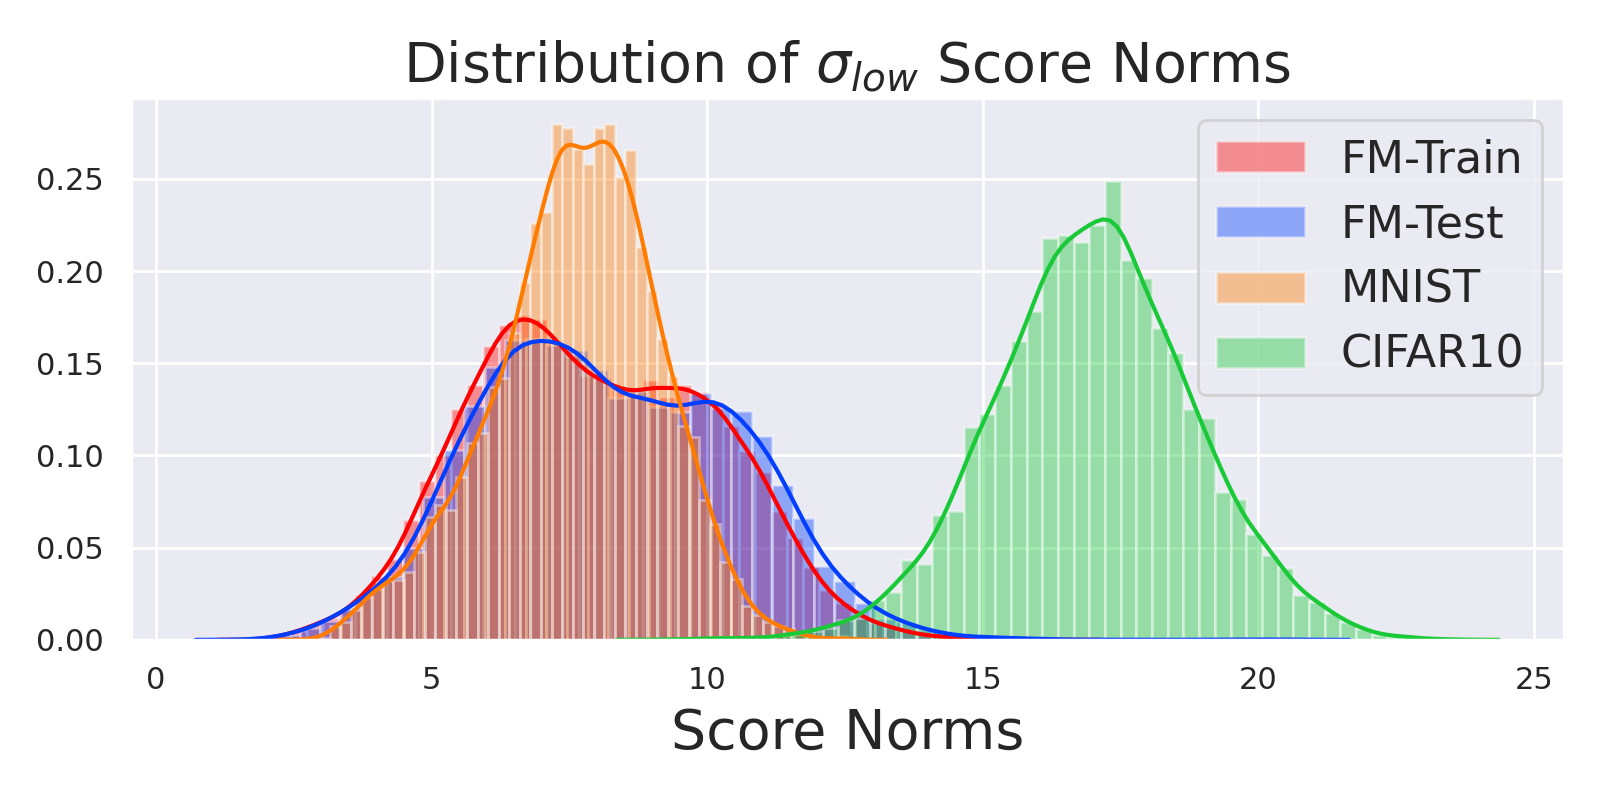
\includegraphics[width=0.9\textwidth]{figures/low_sigma_FvM_tight.png}
    \caption{1D score estimates from a model trained on FashionMNIST (FM)}
    \label{fig:score_norms}
\end{subfigure}
\hfill
\begin{subfigure}[b]{\textwidth}
    \centering
    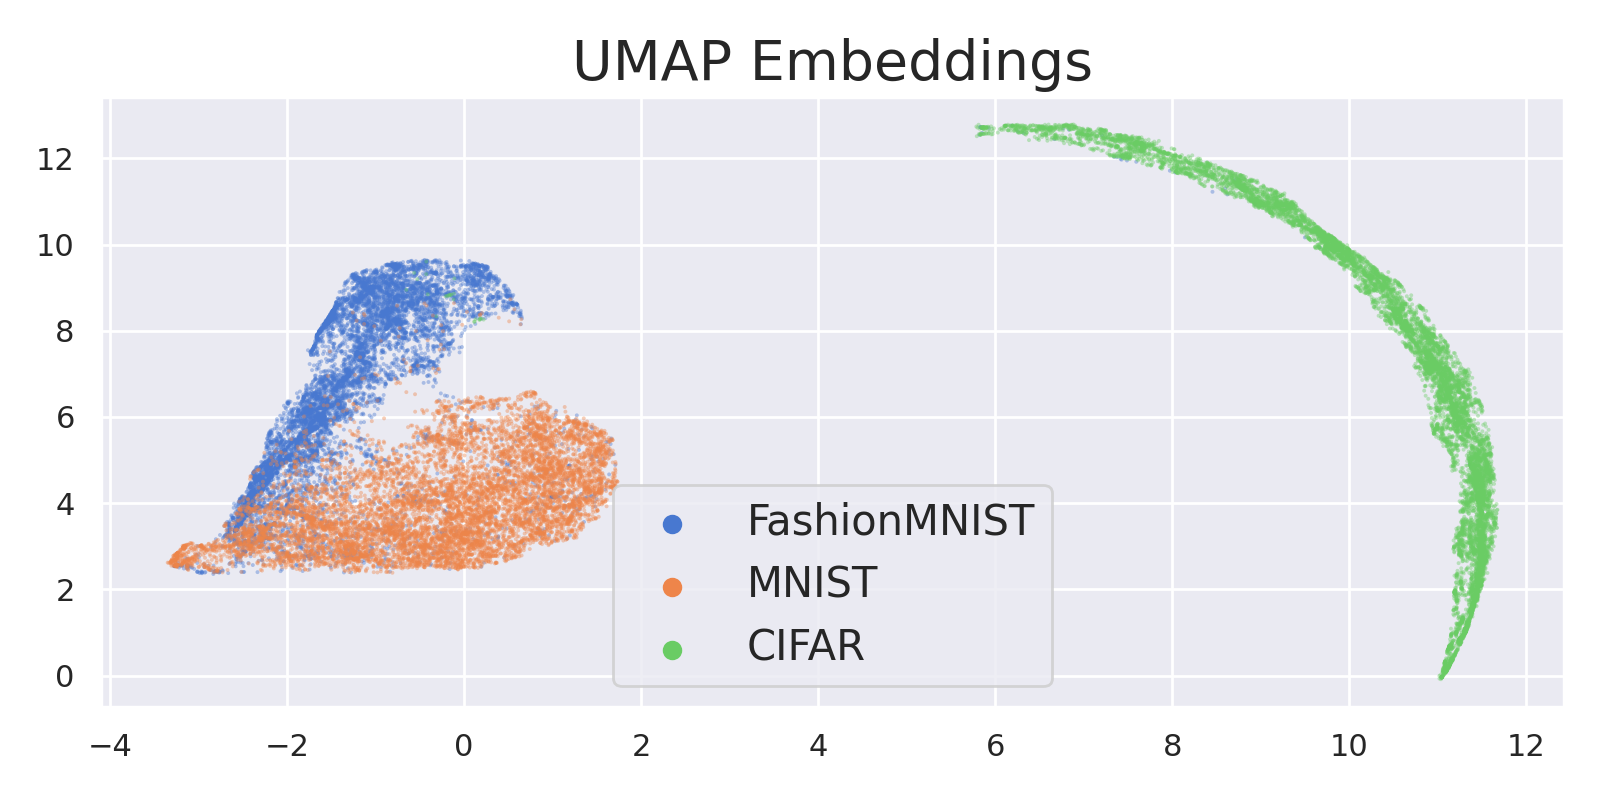
\includegraphics[width=0.9\textwidth]{figures/umap_fashion_tight.png}
    \caption{UMAP visualization of 10-dimensional score estimates from a model trained on FashionMNIST}
    \label{fig:umap}
\end{subfigure}

\caption{Visualizing the need for a multiscale analysis. In (a), I plot the scores corresponding to the lowest sigma estimate. In (b), I plot the UMAP embedding of the $L=10$ dimensional vectors of score norms. Here we see a better separation between FashionMNIST and MNIST when using estimates from \textit{multiple} scales rather than the one that corresponds to the true score only.}
\end{figure}


\subsection*{Why Do Multiscale Scores Capture Outliers?}
\label{neighborhoods}
%TODO: Have arrows pointing showing gradients 
\begin{figure}[tbhp]
\centering
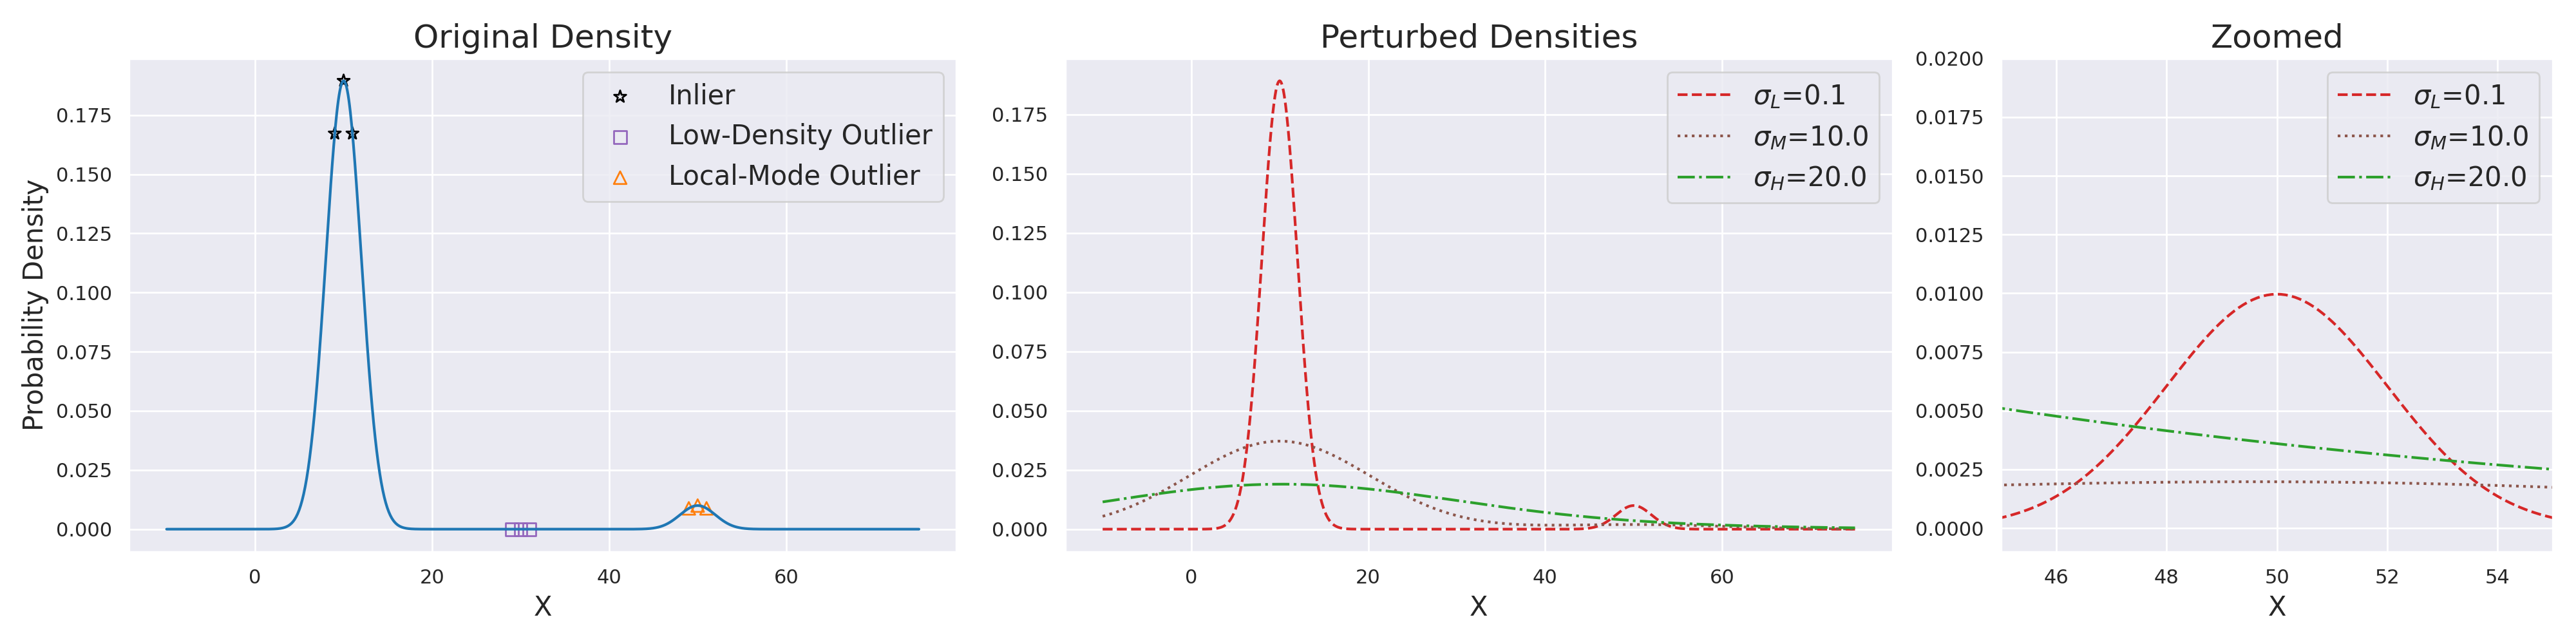
\includegraphics[width=\linewidth]{figures/gmm_plot_tight.png}
\caption{Left: A toy GMM to visualize my analysis with the three regions of interest. Right: Gaussian perturbed versions of the original distribution with (L)ow, (M)edium, and (H)igh noise levels, along with a plot zoomed into the local-mode outliers. Note the effect of different scales on this region: only the largest scale results in a gradient in the direction of the inliers.}
\label{fig:toygmm}
\end{figure}

 In this section, I present an analysis in order to give an intuition for why multiple scales can be useful for OOD detection. Consider the toy distribution shown in \figref{fig:toygmm}. We have three regions of interest: an inlier region with high density centered around $x=10$, an outlier region with low density around $x=30$, and a second outlier region with a local mode centered around $x=50$. I will be adding noise of increasing scales to this distribution and observing the resulting score norms.

To begin, recall that sum of two probability distributions is equivalent to a convolution of their probability density functions, as per the law of total probability~\cite{sumisconv}. Thus, I can analytically compute the perturbed distribution, as I know the parameters for both the base distribution (a Gaussian Mixture Model) and the noise $\mathcal{N}(0; \sigma_i)$. 
This not only enables us to visualize perturbations of our toy distribution, but also to analytically compute the score estimates given any $\sigma_i$.

On the left hand side, we have the initial density with no perturbation. Note how points within the low-density region and at the peak of the local-mode will have small gradients due to being inside a flat area. As we perturb the samples, we smooth the original density, causing it to widen. The relative change in density at each point is dependent on neighboring modes. A large scale perturbation will proportionally take a larger neighborhood into account at each point of the convolution. Therefore, at a sufficiently large scale, nearby outlier points gain context from in-distribution modes. This results in an increased gradient signal in the direction of inliers. 

\begin{figure}[tbhp]

\centering
\begin{subfigure}[b]{0.45\textwidth}
    \centering
    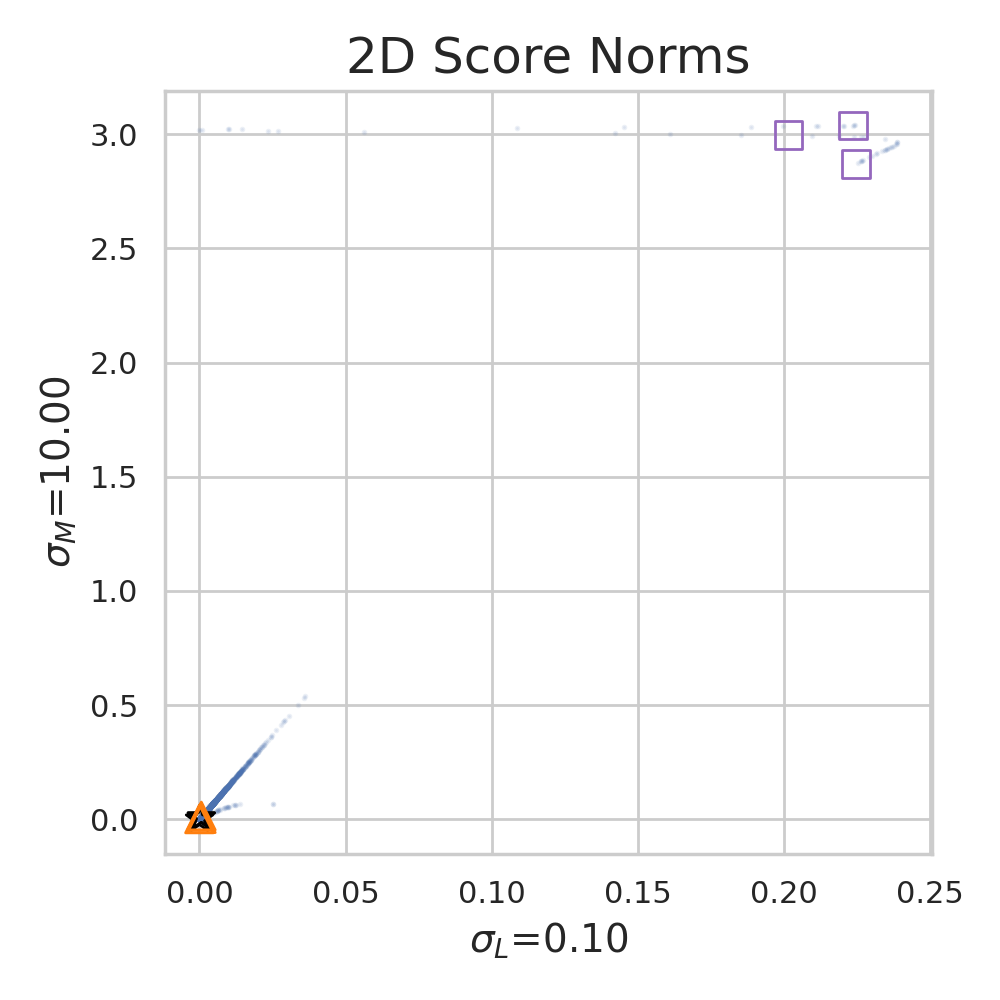
\includegraphics[scale=0.3]{figures/scatter_2d_white.png}
    % \caption{}
    \label{fig:score_norms_2d}
\end{subfigure}
% \hfill
\begin{subfigure}[b]{0.45\textwidth}
    \centering
    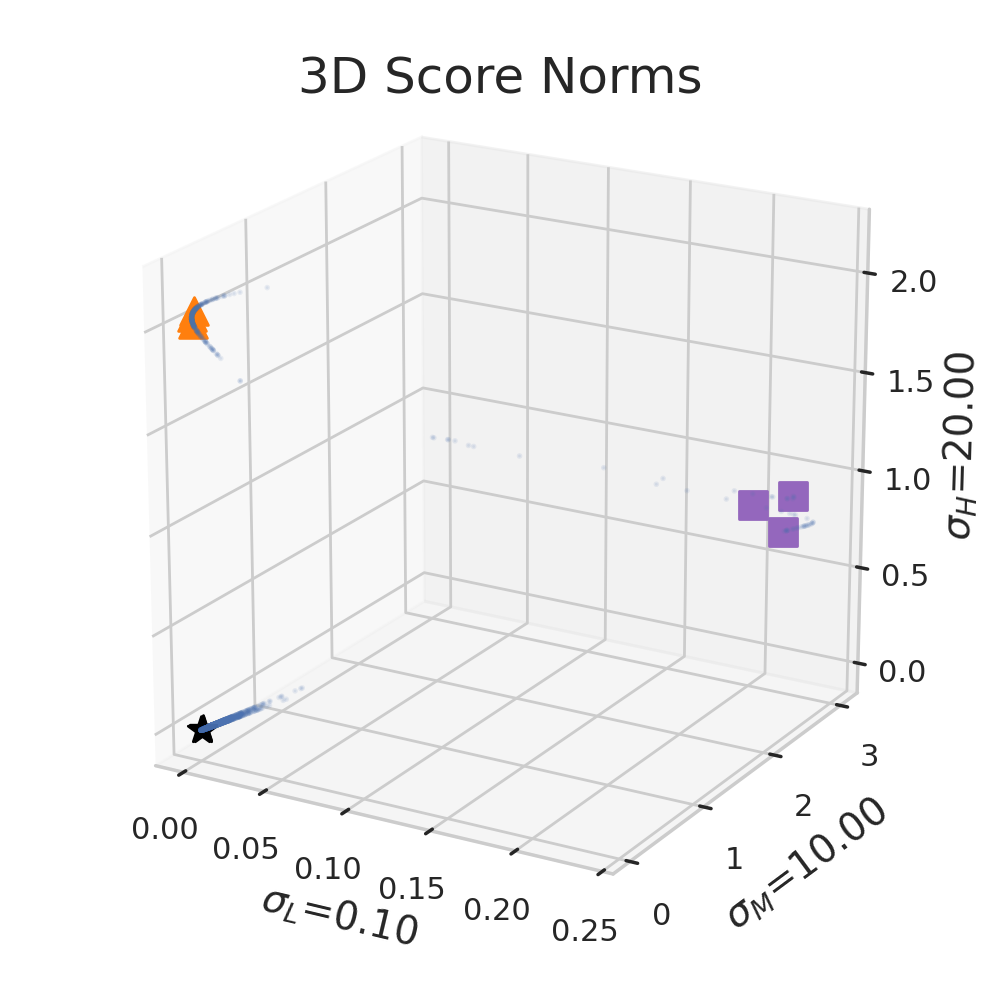
\includegraphics[scale=0.3]{figures/scatter_3d_white.png}
    % \caption{}
    \label{fig:score_norms_3d}
\end{subfigure}
\caption{In (a) observe that Low-Density outliers have comparatively high gradient norms for both $\sigma_{L}$ and $\sigma_{M}$. However at this scale, Local-Mode points still have very small norms, causing them to be tightly packed around the in-distribution points. In (b) we see that Local-Mode outliers achieve a gradient signal only when a sufficiently high scale is used, $\sigma_{H}=20$.}
\label{fig:norm_plots}
\end{figure}

Figure~\ref{fig:norm_plots} plots the score norms of samples generated from the original density along with markers indicating our key regions. Note how a small scale perturbation ($\sigma_{L}=0.1$) stays very close to the true distribution. A medium scale ($\sigma_{M}=10$) Gaussian perturbation is wide enough to ``capture" the Low-Density outliers but still not wide enough to reach the inlier region from the Local-Mode outlier densities, causing them to simply fade into flat nothingness. It is only after we perform a large scale ($\sigma_{H}=20$) perturbation that the in-distribution mode gets taken into account, resulting in a higher gradient norm. This analysis allows one to intuit that larger noise levels account for a larger neighborhood context. We surmise that given a sufficiently large scale, we can capture gradient signals from distant outliers.

\subsection*{Are Larger Scales Always Better?}

However, it is imperative to note that no single scale is guaranteed to work for \textit{all} outliers. Consider outliers close to inlier modes such as the samples between Low-Density outliers and Inliers in \figref{fig:toygmm}. $\sigma_H$ results in an overlap in the score distribution of inliers and Low-Density outliers. This makes it difficult to differentiate the aforementioned ``in-between" outliers from the in-distribution samples. However, this large scale was necessary to get a big enough neighborhood context in order to capture the more distant Local-Mode outliers. Therefore, I postulate that a \emph{range} of scales is necessary for separating outliers.

Admittedly, selecting this range according to the dataset is not a trivial problem. \cite{song2020improved} outlined some techniques for selecting $\{\sigma_i\}_{i=1}^L$ for NCSNs from the perspective of generative modeling. Perhaps there is a similar analog to OOD detection. I did not perform such a statistical analysis for this work and used the default range for NCSN in all my experiments. However, I observed that my defaults are surprisingly generalizable, evident by the fact that all my experiments in Section~\ref{experiments} were performed with the same scale range. In Section~\ref{hyperparams}, I further analyze how varying the scale range effects downstream accuracy and observe that the defaults were already near optimal.


\section{Training an MSMA Model}

I propose the inclusion of multiple noisy score estimates for the task of separating in- and out-of-distribution points, allowing for a Multiscale Score Matching Analysis (MSMA). Concretely, given $L$ noise levels, we calculate the L2-norms of per-sample scores for each level, resulting in an $L$-dimensional vector for each input sample. Motivated by my analyses in Section~\ref{multiscale}, I posit that in-distribution data points occupy distinct and dense regions in the $L$-dimensional score space.

The \textit{cluster assumption} states that decision boundaries should not pass high density regions, but instead lie in low density regions. This implies that any auxiliary method trained to learn in-distribution regions should be able to identify OOD data points that reside outside the learned space. Thus, I propose a two step unsupervised training scheme. First, one trains a NCSN model $s_{\text{IN}}(x, \sigma_L)$ to estimate scores for inlier samples, given $\{\sigma_i\}_{i=1}^L$ levels of noise. Next, we can calculate all $L$ noisy score estimates for the $N$ training samples and take the L2-norms across the input dimensions: $[\norm{  s_{\text{IN}} (X, \sigma_1) }_2^2, ... , \norm{  s_{\text{IN}} (X, \sigma_L) }_2^2 ]$. This results in an $N$x$L$ matrix. Finally, we can train an auxiliary model (such as a Gaussian Mixture Model) on this matrix to learn the spatial regions of in-distribution samples in the $L$-dimensional space.

\subsection*{Learning Concentration in the Score Space}

We posit that learning the ``density" of the inlier data in the $L$-dimensional score (norm) space is sufficient for detecting out-of-distribution samples. The term “density” can be interpreted in a myriad of ways. I primarily focus on models that fall under three related but distinct notions of denseness: spatial clustering, probability density, and nearest (inlier) neighbor graphs. All three allow us to threshold the associated metric to best separate OOD samples.

Spatial clustering is conceptually the closest to our canonical understanding of denseness: points are tightly packed under some metric (usually Euclidean distance). Ideally OOD data should not occupy the same cluster as the inliers. I train Gaussian Mixture Models (GMMs) to learn clusters in the inlier data. GMMs work under the assumption that the data is composed of k-components whose shapes can be described by a (multivariate) Gaussian distribution. Thus for a given datum, one can calculate the joint probability of it belonging to any of the k-components.

Probability density estimation techniques aim to learn the underlying probability density function $p_{data} (x)$ which describes the population. Normalizing flows are a family of flexible methods that can learn tractable density functions (\cite{Papamakarios2019}). They transform complex distributions into a simpler one (such as a Gaussian) through a series of invertible, differential mappings. The simpler base distribution is then used to infer the density of a given sample. For this work, I use Masked Autoregressive Flows introduced by \cite{Papamakarios2017masked}, which utilizes neural networks as the transformation functions. The inlier likelihoods are used to determine a threshold after which samples are considered outliers.

Finally, I consider k-nearest neighbor (k-NN) graphs to allow for yet another thresholding metric. Conceptually, the idea is to sort all samples according to distances to their k-closest (inlier) neighbor. Presumably, samples from the same distribution as the inliers will have very short distances to training data points. Despite its simplicity, this method is surprisingly accurate. It is also computationally efficient as k-NN distances can be computed via efficient data structures (such as KD Trees).


\section{Experiments on Benchmark Datasets}
\label{experiments}

In this section I demonstrate MSMA's potential as an effective OOD detector. I first train a NCSN model as my score estimator, and then an auxiliary model on the score estimates of the training set. Following \cite{Liang2017} and \cite{Devries}, I use CIFAR-10 and SVHN as my “inlier” datasets alongside a collection of natural images as "outlier" datasets. I retrieve the natural image from ODIN's publicly available GitHub repo\footnote{\url{https://github.com/facebookresearch/odin}}. This helps maintain a fair comparison (e.g. it ensures I test the same random crops as ODIN). I will denote \cite{Liang2017} as ODIN and \cite{Devries} as Confidence in my tables.
In addition to experiments performed by \cite{Hendrycks2019}, \cite{Liang2017} and \cite{Devries}, I also distinguish \textit{between} CIFAR and SVHN and compare my results to baselines.

% Additionally, I report our results for FashionMNIST vs MNIST in Section~\ref{fashion_exp}.


\subsection*{Datasets}
\label{datasets}
I consider CIFAR-10 (\cite{Krizhevsky2009learning}) and SVHN (\cite{Netzer2011reading}) as my inlier datasets. For out-of-distribution datasets, I choose the same as \cite{Liang2017}: \textbf{TinyImageNet}\footnote{\url{https://tiny-imagenet.herokuapp.com/}}, \textbf{LSUN} (\cite{Yu2015lsun}), \textbf{iSUN} (\cite{Xu2015turkergaze}). Similar to \cite{Devries}, in my main experiments I report only \textit{resized} versions of \textit{LSUN} and \textit{TinyImageNet}. I also leave out the synthetic \textbf{Uniform} and \textbf{Gaussian} noise samples from my main experiments as I performed extremely well in all of those experiments.
% We refer the reader to \ref{full_baselines} for the full report including all datasets.

Lastly following \cite{Devries}, I consider \textbf{All Images}: a combination of all non-synthetic OOD datasets outlined above (including \textit{cropped} versions). Note that this collection effectively requires a single threshold for all datasets, thus arguably reflecting a real world out-of-distribution setting.

\subsection*{Evaluation Metrics}

To measure thresholding performance it is common to use the metrics established by previous baselines (\cite{Hendrycks2019}, \cite{Liang2017}). These include:

\textbf{FPR at 95\% TPR:} This is the False Positive Rate (FPR) when the True Positive Rate (TPR) is 95\%. This metric can be interpreted as the probability of misclassifying an outlier sample to be in-distribution when the TPR is as high as 95\%. Let TP, FP, TN, and FN represent true positives, false positives, true negatives and false negatives respectively. FPR=FP/(FP+TN), TPR=TP/(FN+TP).

\textbf{Detection Error:} This measures the minimum possible misclassification probability over all thresholds. Practically this can be calculated as $\min_{\delta} 0.5(1-\text{TPR}) + 0.5\text{FPR}$, where it is assumed that we have an equal probability of seeing both positive and negative examples in the test set.

\textbf{AUROC:} This measures area under (AU) the Receiver Operating Curve (ROC) which plots the relationship between FPR and TPR. It is commonly interpreted as the probability of a positive sample (in-distribution) having a higher score than a negative sample (out-of-distribution). It is a threshold independent, summary metric.

\textbf{AUPR:} Area Under the Precision Recall Curve (AUPR) is another threshold independent metric that considers the PR curve, which plots Precision(= TP/(TP+FP) ) versus Recall(= TP/(TP+FN) ). AUPR-In and AUPR-Out consider the in-distribution samples and out-of-distribution samples as the positive class, respectively. This helps take mismatch in sample sizes into account.

\subsection*{Comparison Against Previous OOD Methods}
\label{ood_experiments}

I compare my work against Confidence Thresholding (\cite{Devries}) and ODIN (\cite{Liang2017}). For all experiments I report the results for the in-distribution \textit{testset} vs the out-of-distribution datasets. Note that \textit{All Images*} is a version of \textit{All Images} where both ODIN and Confidence Thresholding perform input preprocessing. Particularly, they perturb the samples in the direction of the softmax gradient of the classifier:
$\tilde{x} = x - \epsilon \text{ sign} (- \nabla_x log S_y(x;T))$.
They then perform a grid search over $\epsilon$ ranges, selecting the value that achieves best separation on 1000 samples randomly held for \textit{each} out-of-distribution set. ODIN performs an additional search over $T$ ranges, while Confidence Thresholding uses a default of $T=1000$. I did not perform any such input modification. Note that ODIN uses input thresholding for individual OOD datsets as well, while Confidence Thresholding does not. 

My results show that MSMA clearly outperforms baselines as reported in Table~\ref{msma_results}. For brevity, only report \textbf{ FPR (95\% TPR)} and \textbf{AUROC}. All other metric comparisons are reported in the Section~\ref{msma_extended_results}. 

\begin{table}[htbp]
\label{msma_results}
\small
\centering
% \def\arraystretch{1.1}
\begin{tabular}{>{\centering}m{0.55in} >{\raggedright}p{0.85in} *{4} {>{\centering}m{0.55in}} * {1} {>{\centering\arraybackslash}m{0.65in}}}
\hline
\begin{tabular}[c]{@{}c@{}}Dataset\end{tabular} & 
\begin{tabular}[c]{@{}c@{}}OOD\\ Dataset\end{tabular} & 
\begin{tabular}[j]{@{}c@{}}GMM\\ MSMA \end{tabular} &
\begin{tabular}[j]{@{}c@{}}Flow\\ MSMA \end{tabular} & 
\begin{tabular}[j]{@{}c@{}}KD Tree \\MSMA\end{tabular} &
\begin{tabular}[j]{@{}c@{}}ODIN \end{tabular} &
\begin{tabular}[j]{@{}c@{}}Confidence \end{tabular} \\ \hline
% & \multicolumn{5}{c}{FPR / AUROC}

         & TinyImageNet
          & \textbf{0} / \textbf{100.0}   & \textbf{0} / \textbf{100.0}   & \textbf{0} / \textbf{100.0}  & -    & 1.8 / 99.6  \\  
          & LSUN           
          & \textbf{0} / \textbf{100.0}   & \textbf{0} / \textbf{100.0}   & \textbf{0} / \textbf{100.0}  & -          & 0.8 / 99.8 \\  
SVHN      & iSUN           
          & \textbf{0} / \textbf{100.0}   & \textbf{0} / \textbf{100.0}   & \textbf{0} / \textbf{100.0}  & -          & 1.0 / 99.8 \\ 
          & All Images     
          & \textbf{0} / \textbf{100.0}   & \textbf{0} / \textbf{100.0}   & \textbf{0} / \textbf{100.0}  & -          & 4.3 / 99.2 \\
          & All Images*    & -             & -             & -            & 8.6 /97.2 & 4.1 / 99.2 \\ \hline

          & TinyImageNet   
          & \textbf{0} / \textbf{100.0}   & \textbf{0} / \textbf{100.0}   & 0.3 / 99.9   & 7.5 / 98.5   & 18.4 / 97.0  \\  
          & LSUN           
          & \textbf{0} / \textbf{100.0}   & \textbf{0} / \textbf{100.0}   & 0.6 / 99.9   & 3.8 / 99.2   & 16.4 / 97.5 \\  
CIFAR-10     & iSUN           
          & \textbf{0} / \textbf{100.0}   & \textbf{0} / \textbf{100.0}   & 0.4 / 99.9   & 6.3 / 98.8   & 16.3 / 97.5 \\
          & All Images     
          & \textbf{0} / \textbf{100.0}   & \textbf{0} / \textbf{100.0}   & 0.4 / 99.9   & -            & 19.2 / 97.1 \\
          & All Images*    & -             & -             & -            & 7.8 / 98.4   & 11.2 / 98.0 \\ \hline
\end{tabular}%\hspace*{-0.1\textwidth}
\caption{Comparing our auxiliary methods against existing state-of-the-art. \textbf{FPR (95\% TPR)} (\textit{Lower} is better)/ \textbf{AUROC} (\textit{Higher} is better). MSMA methods unequivocally outperform previous work in all tests, with KD Trees only slightly worse than GMM and Flow variants.}
\end{table}

\begin{table}[tbhp]
\small
\centering
% \def\arraystretch{1.2}
\begin{tabular}{>{\centering}m{0.5in} >{\centering}m{0.6in} >{\centering}m{0.5in} *{3} {>{\centering\arraybackslash}m{0.4in}}}
\hline
\begin{tabular}[c]{@{}c@{}}Auxiliary\\ Method\end{tabular} & 
\begin{tabular}[j]{@{}c@{}}FPR\\ (95\% TPR)\\ $\downarrow$ \end{tabular} &
\begin{tabular}[j]{@{}c@{}}Detection\\ Error\\ $\downarrow$ \end{tabular} & 
\begin{tabular}[j]{@{}c@{}}AUROC\\ \\$\uparrow$\end{tabular} &
\begin{tabular}[j]{@{}c@{}}AUPR\\ In\\ $\uparrow$\end{tabular} &
\begin{tabular}[j]{@{}c@{}}AUPR\\ Out\\ $\uparrow$\end{tabular} \\ \hline


GMM       & 11.4   & 8.1     & 95.5    & 91.9     & 96.9 \\ \hline
 
Flow      & 8.6    & 6.8     & 96.7    & 93.4     & 97.7 \\  \hline

KD Tree   & \textbf{4.1}   & \textbf{4.5}    & \textbf{99.1}   & \textbf{99.1}     & \textbf{99.2} \\ \hline
\end{tabular}%\hspace*{-0.1\textwidth}

\caption{Comparison of auxiliary models tasked to separate CIFAR-10 (in-distribution) and SVHN (out-of-distribution). $\downarrow$ indicates lower values are better and $\uparrow$ indicates higher values are better.}
\label{cifar_perf}
\end{table}

\begin{table}[tbhp]
\small
\centering
\begin{tabular}{*{2} {>{\centering}m{1.0in}} *{4} {>{\centering\arraybackslash}m{0.55in}}}
\hline
\begin{tabular}[j]{@{}c@{}}Detection \\ Function\end{tabular} & 
\begin{tabular}[j]{@{}c@{}}Model \end{tabular} & 
            % FPR (95\% TPR) & AUROC    & AUPR In  & AUPR Out \\ \hline
\begin{tabular}[j]{@{}c@{}}FPR\\ (80\% TPR)\\ $\downarrow$ \end{tabular} &
\begin{tabular}[]{@{}c@{}}AUROC\\ \\ $\uparrow$\end{tabular} &
\begin{tabular}[]{@{}c@{}}AUPR\\ In\\ $\uparrow$\end{tabular} &
\begin{tabular}[]{@{}c@{}}AUPR\\ Out\\ $\uparrow$\end{tabular} \\ \hline

$||s_{\theta} (x, \sigma_i^L)||$              & KD Tree MSMA
& \textbf{0.7 }  & \textbf{99.1}      & \textbf{99.1 }    & \textbf{99.2} \\

$\log \frac{p_{\theta}(x)}{p_{\theta_0}(x)}$  & Likelihood Ratios
& 6.6   & 93.0      & 88.1    & -  \\ 

$\log p(x)$       & JEM                   
& -     & 67.0       & -     & -\\ 

$\norm{ \frac{\partial \log p(x)}{\partial x}}$       & Approx. Mass JEM  
& -     & 83.0      & -     & - \\ \hline
\end{tabular}\hspace*{-0.1\textwidth}

\caption{Comparison with a multitude of likelihood-based models at separating CIFAR-10 (in-distribution) from SVHN (out-of-distribution). - represent metrics that were not reported by the work.  All values are shown in percentages. $\downarrow$ indicates lower values are better and $\uparrow$ indicates higher values are better. Note that since Likelihood Ratios report FPR at \textbf{80\%} TPR, we report the same.}
\label{likelihoods}

\end{table}

\subsection*{MSMA Succeeds where Likelihoods Fail}

\cite{nalisnick2018do} showed how deep generative models are particularly inept at separating high dimensional complex datasets such as these two. One exemplary experiment kept CIFAR-10 as in-distribution and SVHN as out-of-distribution. It is common for researchers to use this experiment to explore the OOD failure of likelihood models~\cite{why_norm_fails,Ren2019,Grathwohl2020Your}. Since this setting is not considered in the testbed used by ODIN or Confidence Thresholding, I did not report their results. 

Table~\ref{cifar_perf} shows MSMAs performance for this task. Note that \textit{all} three auxiliary models definitively outperform the baselines (see Table~\ref{likelihoods}), with KD-Trees preforming the best. Likelihood Ratios~\cite{Ren2019}, and JEM~\cite{Grathwohl2020Your} are two unsupervised methods that have tackled this problem and have reported current state-of-the-art results. Table~\ref{likelihoods} summarizes the results that were reported by these papers. Both report AUROCs, with \cite{Ren2019} additionally reporting AUPR(In) and FPR at 80\% TPR. Since each method proposes a different detection function, we also provide them for reference.
\goodbreak

\section{Case Study: Age based OOD Detection from Brain MRI Scans}
\label{brain_experiment}

In this section I report MSMA's performance on a real-world case study. Here the task is to detect brain Magnetic Resonance Images (MRIs) from pediatric subjects at an age (1 - 6 years) that is younger than the inlier data (9 - 11 years of age). We expect visible differences in image contrast and local brain morphometry between the brains of a toddler and an adolescent. As a child grows, their brain matures and the corresponding scans appear more like the prototypical adult brain. This provides an interesting gradation of samples being considered out-of-distribution with respect to age.

I employ 3500 high resolution T1-weighted MR images obtained through the NIH large scale ABCD study~\cite{Casey2018adolescent}, which represent data from the general adolescent population (9-11 years of age). This implies that my in-distribution dataset will have high variation. After standard preprocessing, we extracted for each dataset three mid-axial slices and resized them to be 90x110 pixels, resulting in $\sim$11k axial images (10k  training, 1k testing). For my outlier data, we employ MRI datasets of children aged 1, 2, 4 and 6 years (500 each) from the UNC EBDS database \cite{Stephens:2020bo,Gilmore:2020ct}.
\begin{figure}[tbhp]
\centering
\begin{subfigure}[b]{0.22\textwidth}
    % \centering
    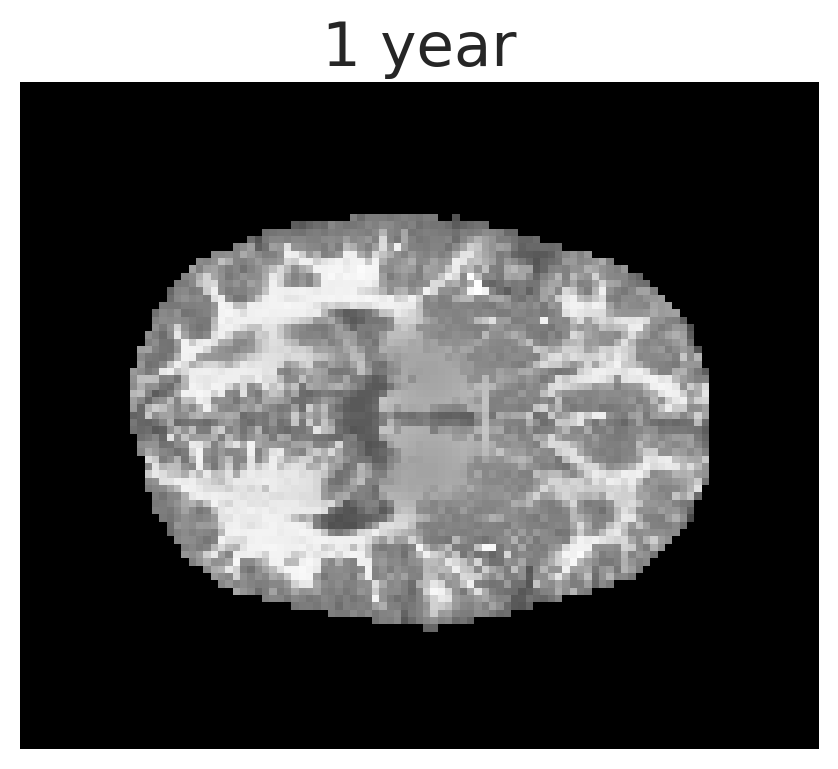
\includegraphics[width=\textwidth]{figures/1_year.png}
    % \caption{}
    \label{fig:brain_1}
\end{subfigure}
\begin{subfigure}[b]{0.22\textwidth}
    % \centering
    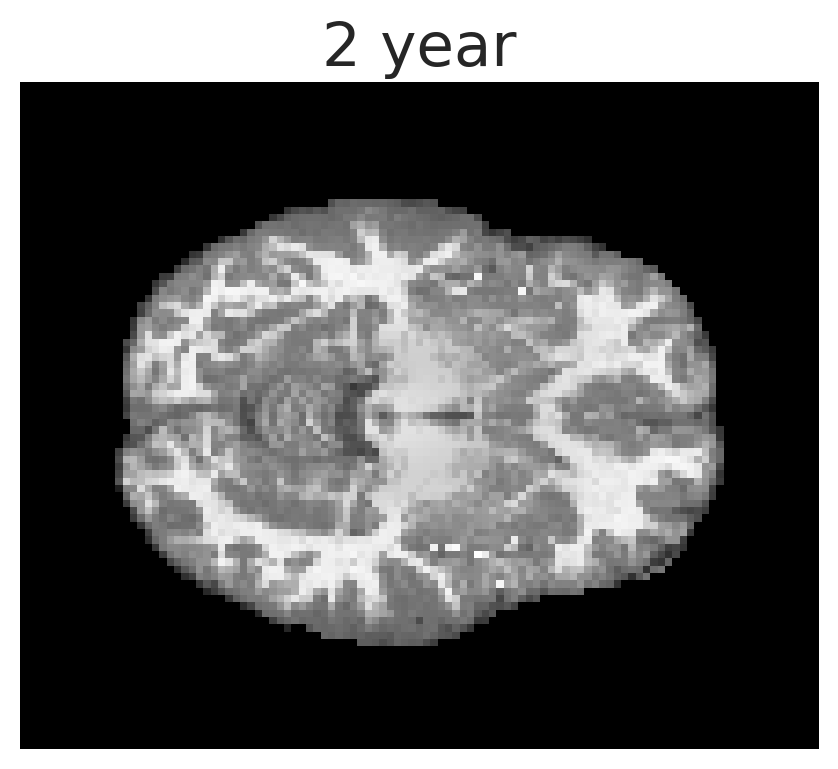
\includegraphics[width=\textwidth]{figures/2_year.png}
    % \caption{}
    \label{fig:brain_2}
\end{subfigure}
\begin{subfigure}[b]{0.22\textwidth}
    % \centering
    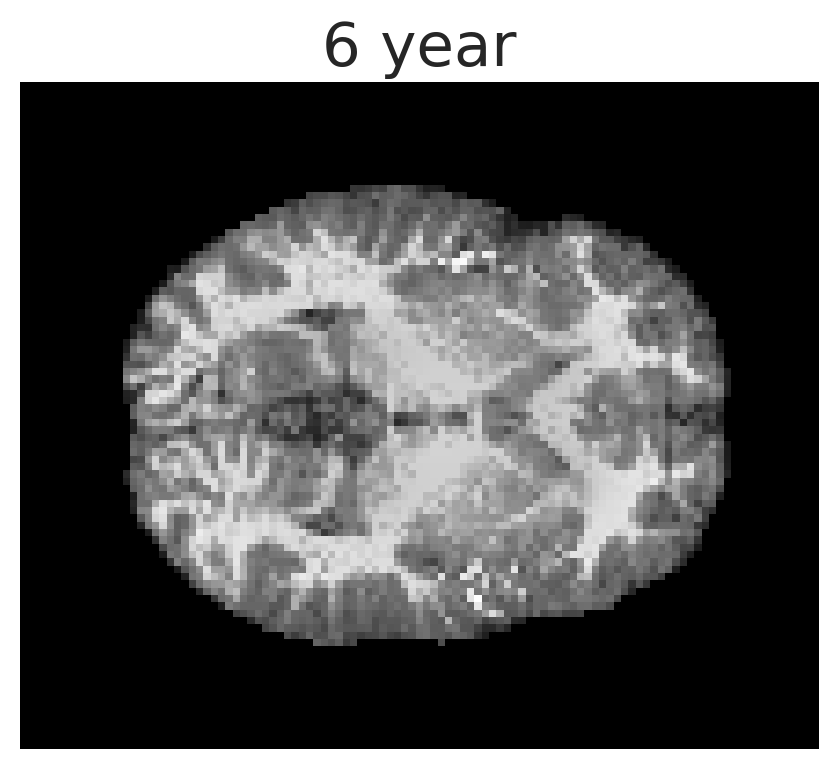
\includegraphics[width=\textwidth]{figures/6_year.png}
    % \caption{}
    \label{fig:brain_3}
\end{subfigure}
\begin{subfigure}[b]{0.22\textwidth}
    % \centering
    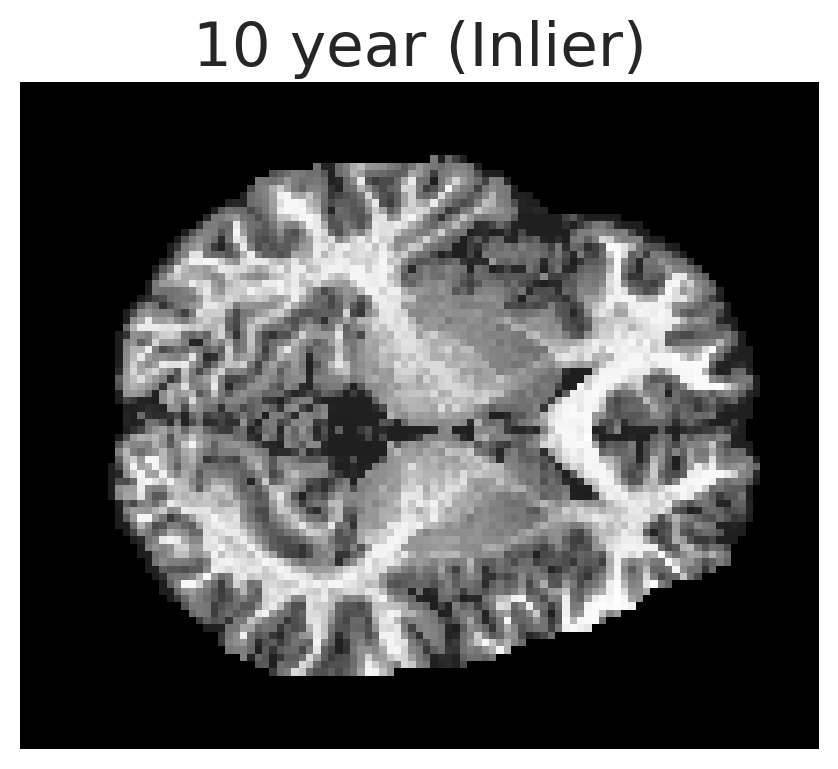
\includegraphics[width=\textwidth]{figures/10_year_lab.png}
    % \caption{}
    \label{fig:brain_4}
\end{subfigure}

\caption{Note the change in image contrast, brain size and brain matter structure as the child grows. Each age is increasingly difficult to distinguish from our inliers.}
\label{fig:brain_plots}
\end{figure}

MSMA was effectively able to identify younger age groups as out-of-distribution. Table~\ref{brain_perf} reports the results for GMMs trained for this task. As expected, the separation performance decreases as age increases. Note that we kept the same hyperparameters for our auxiliary methods as in the previous experiments despite this being a higher resolution scenario. I also note that the Flow model and KD Tree perform equally well and refer the reader to Table~\ref{brain_perf_full} in Section~\ref{msma_extended_results}.

\begin{table}[tbhp]
\small
\centering
\def\arraystretch{1.1}
\begin{tabular}{>{\centering}m{0.65in} >{\centering}m{0.75in} >{\centering}m{0.65in} *{3} {>{\centering\arraybackslash}m{0.85in}}}
\hline
\begin{tabular}[c]{@{}c@{}}OOD Age\\ (Years)\end{tabular} & 
            % FPR (95\% TPR) & AUROC    & AUPR In  & AUPR Out \\ \hline
\begin{tabular}[j]{@{}c@{}}FPR\\ (95\% TPR)\\ $\downarrow$ \end{tabular} &
\begin{tabular}[j]{@{}c@{}}Detection\\ Error\\ $\downarrow$ \end{tabular} & 
\begin{tabular}[j]{@{}c@{}}AUROC\\ \\$\uparrow$\end{tabular} &
\begin{tabular}[j]{@{}c@{}}AUPR\\ In\\ $\uparrow$\end{tabular} &
\begin{tabular}[j]{@{}c@{}}AUPR\\ Out\\ $\uparrow$\end{tabular} \\ \hline
& \multicolumn{5}{c}{f-AnoGAN / MSMA} \\ 
\cline{2-6}
 1               &  94.0 / \textbf{0.2}     &  24.1.0 / \textbf{0.4}     & 72.4 / \textbf{99.9}   & 80.2 / \textbf{99.9 }   & 62.2 / \textbf{99.9} \\  
 2               & 62.7 / \textbf{0.6}    & 13.8 / \textbf{1.0}    & 90.6 / \textbf{99.7}    & 92.5 / \textbf{99.5}     & 87.0 / \textbf{99.9} \\  
 4               & 60.9 / \textbf{23.7}   & 19.0 / \textbf{9.2}    & 87.9 / \textbf{96.1}    & 88.9 / \textbf{93.8}     & 85.8 / \textbf{97.9} \\ 
 6               & 78.1 / \textbf{30.5}   & 31.1 /\textbf{ 9.7}    & 74.6 / \textbf{95.0}    & 76.4 / \textbf{92.2}     & 72.4 / \textbf{96.8} \\ \hline
\end{tabular}

\caption{MSMA-GMM trained on multiscale score estimates tasked to separate the brain scans of different age groups. In-distribution samples are 9-11 years of age. All values are shown in percentages. $\downarrow$ indicates lower values are better and $\uparrow$ indicates higher values are better. The results show that f-AnoGAN is unable to match the performance of MSMA for this task. In fact, under some metrics such as FPR at 95\% TPR, it exhibits very poor performance as an anomaly detector.}

\label{brain_perf}
\end{table}

I compared MSMA to f-AnoGAN~\cite{schlegl2019f} due to its promising results as an anomaly detector and its popularity in the medical community. I use the hyperparameters suggested in the original paper and trained them till convergence. Interestingly, MSMA outperforms f-AnoGAN in \textit{all} experiments. However, f-AnoGAN is a considerably faster method, both in terms of training and inference, and allows for pixel-wise anomalies out of the box. Although, it should be noted that Spatial-MSMA introduced in Chapter~\ref{ch:localizing} will overcome the latter limitation by adding localization capabilities to MSMA.


\section{Hyperparameter Analysis}
\label{hyperparams}

\begin{figure}[tbhp]

\centering
\begin{subfigure}[b]{0.45\textwidth}
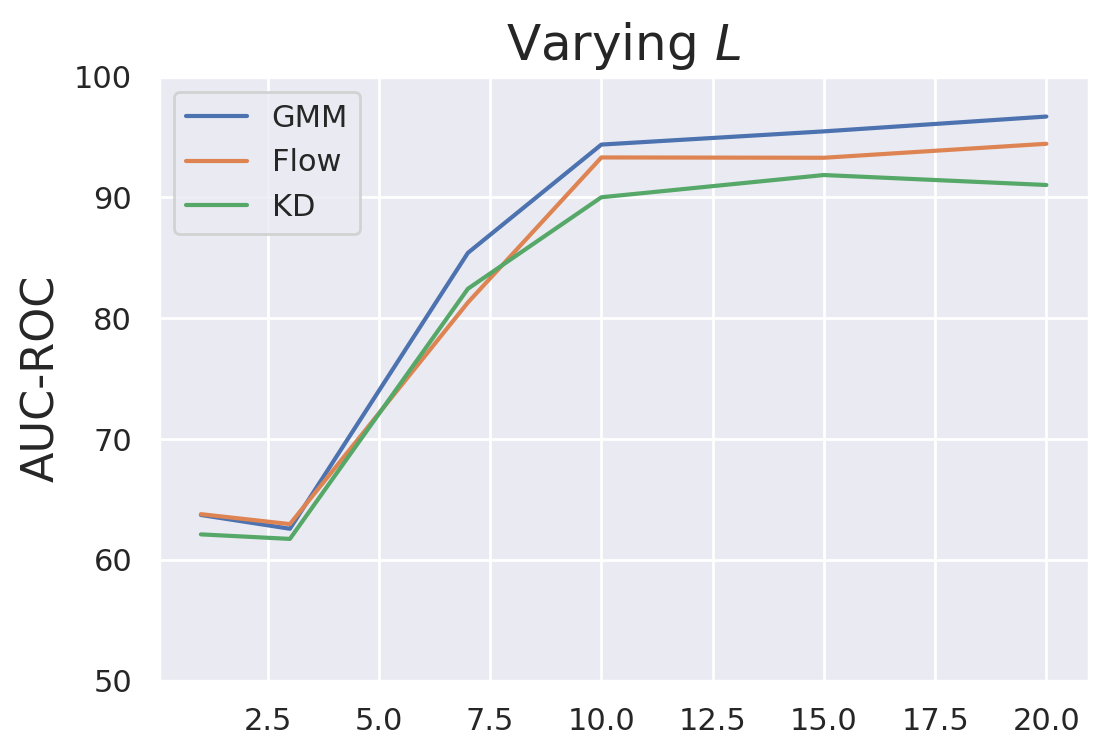
\includegraphics[scale=0.5]{figures/L_analysis.png}
\caption{Varying L from 1 to 20}
\label{fig:L_analysis}
\end{subfigure}
% \hfill
\begin{subfigure}[b]{0.45\textwidth}
    % \centering
    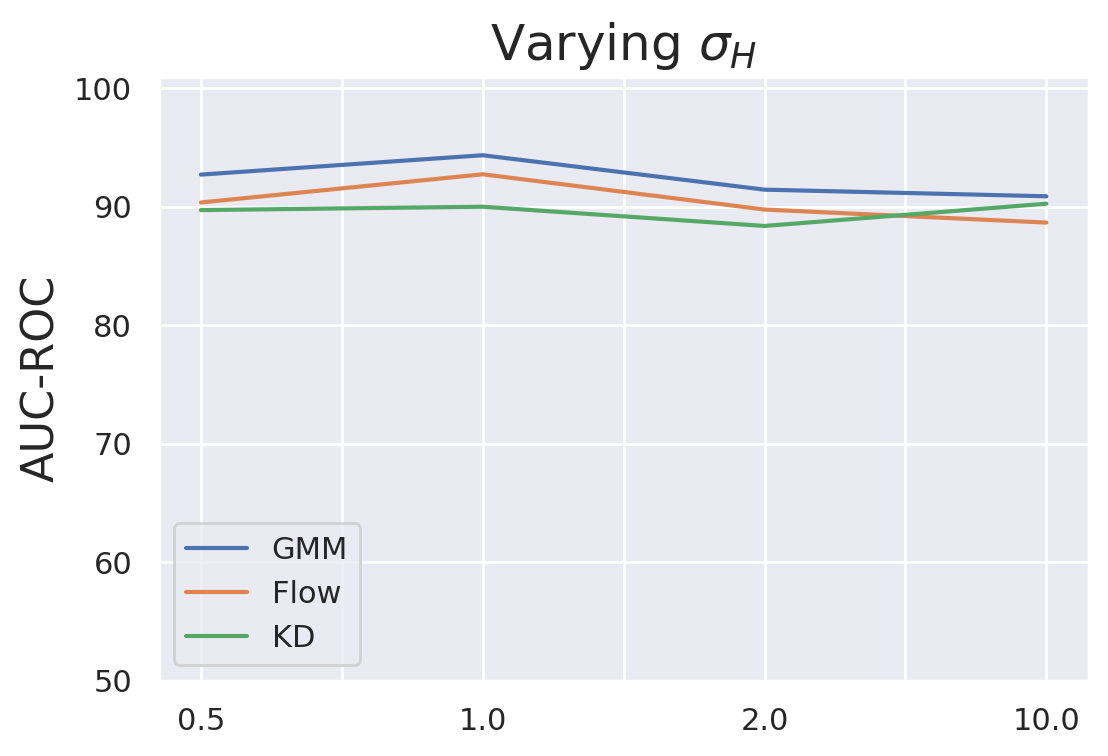
\includegraphics[scale=0.5]{figures/sigma_analysis.png}
    \caption{Varying $\sigma_H$ from 0.5 to 10}
    \label{fig:sigma_analysis}
\end{subfigure}
\caption{Analysis of the effect of hyperparameters $\sigma_H$ and $L$ on MSMA's out-of-distribution detection performance. We observe that the defaults $\sigma=1.0$ and $L=10$ perform the best, with a slight variance in performance when we deviate from them.}
\label{fig:analysis}
\end{figure}


This section explores MSMA's sensitivity to its two main hyperparameters utilized in NCSN: the number of noise levels ($L$) and the largest scale used ($\sigma_H$). The smallest noise scale was fixed to $\sigma_L=0.01$ through all experiments as it is low enough to learn the true score values without running into issues regarding numerical precision. The rationale being that noise perturbations to images at such a small scale are imperceptible to the human eye and are adequate to give an estimate of the true score. For all experiments, I train on CIFAR-10 and evaluate on the \emph{All Images} dataset described in Section~\ref{datasets} and plot AUROC in Figure~\ref{fig:analysis}. In order to reduce GPU memory usage and computation time, I reduced the batch size from 128 to 64, which is why we see a performance dip from the main experiment in Section~\ref{ood_experiments}. The hyperparameters for the auxiliary models are kept the same as the main experiment.

For the number of scales $L$, I tested the values 1, 3, 10, 15, and 20, with $\sigma_H$ fixed at the default value ($\sigma_H=1$). Recall that I follow the original NCSN schema by \cite{Song2019}, and utilize a geometric sequence of sigma scales from $\sigma_H$ to $\sigma_L$ with $L$ steps (endpoint inclusive). Thus, changing \emph{L} changes the intermediate noise scales. The results in Figure~\ref{fig:L_analysis} show that MSMA is optimal near the default ($L=10$). Increasing $L$ does not significantly vary the performance, while small values such as $L=3$ are not adequate at providing enough intermediate scales. Note that $L=1$ is the degenerate case where only the largest noise scale is used. This highlights the need for a range of scales as argued in Section \ref{neighborhoods} and empirically shows that simply using one large scale is not enough. \figurename{~\ref{fig:sigma_analysis}} plots the affect of varying the largest noise scale $\sigma_H$. I test the values 0.5, 1.0, 2.0, and 10, with the default number of scales $L=10$. Again, we observe that our default $\sigma_H=1$ performs the best and there is no noticeable improvement from varying it. Considering how images are rescaled to [0,1] before they are passed to the network, we posit that $\sigma_H=1.0$ already introduces large noise, and increasing it further seems to degrade results to varying degrees. 

Lastly, I would like to emphasize that \emph{all} of my main out-of-distribution experiments in Section~\ref{experiments} were performed with the \emph{same} default hyperparameters, without any tuning. Despite this disadvantage, MSMA still outperforms its competitors ODIN~\cite{Liang2017}, Confidence Thresholding (\cite{Devries}), and Likelihood Ratios~\cite{Ren2019}, all of which need some fine-tuning of hyperparameters. Recognize that tuning requires apriori knowledge of the type of out-of-distribution samples the user expects. From the analysis in this section and my main experiment, \textit{I can confidently advocate the use of MSMA's defaults as they generalize across datasets and do not require such apriori knowledge.} 

% Of course, if anomalies are known at training time then one may tune MSMA's hyperparameters to for the optimal threshold. However, I did not do such finetuning as this Chapter is mainly concerned with introducing MSMA as a performant, easy to implement, and generalizable out-of-distribution detector.

\section{Discussion}

This chapter introduced MSMA: a method based on multiscale score matching. I outlined how scaling the noise perturbation is analogous to the increased context from local neighborhoods in the data space.  


I demonstrated how MSMA outperforms baseline methods in \textit{every} metric for \textit{all} benchmark experiments. MSMA is easy to implement, trains completely unsupervised, requires minimal hyperparameter tuning, and generalizes to many OOD tasks.

The excellent results reported in this chapter empirically validate MSMA as a fast, general purpose anomaly detector. The following chapters will focus on extending MSMA and applying it to 3D MRI data for detecting neurodevelopmental disorders.

\section{Extended Tabulated Results}
\label{msma_extended_results}

This section contains the tables for the extended results. It reports accuracy metrics for three different auxiliary models: Gaussian Mixture Model (GMM), Normalizing Flow density estimator (Flow), and a nearest-neighbour-based model (KD Tree). The purpose of reporting results from different models is to showcase the flexibility of my approach. Each auxiliary model provides a different notion of "distance" from the inliers. A user can choose a downstream model according to their data needs. For instance, a tree-based model can be computationally efficient for high dimensional datasets, compared to the density-based models.

\begin{table}[tbhp]
\label{fpr}
\small
% \def\arraystretch{1.2}
\begin{tabular}{>{\centering}m{0.8in} >{\raggedright}p{0.8in} *{3} {>{\centering}m{0.4in}} * {2} {>{\centering\arraybackslash}m{0.7in}}}
\hline
\begin{tabular}[c]{@{}c@{}}In-distribution\\ Dataset\end{tabular} & 
\begin{tabular}[c]{@{}c@{}}OOD\\ Dataset\end{tabular} & 
\begin{tabular}[j]{@{}c@{}}GMM \end{tabular} &
\begin{tabular}[j]{@{}c@{}}Flow \end{tabular} & 
\begin{tabular}[j]{@{}c@{}}KD \\ Tree\end{tabular} &
\begin{tabular}[j]{@{}c@{}}ODIN \\ (DenseNet) \end{tabular} &
\begin{tabular}[j]{@{}c@{}}Confidence\\ (VGG13)\end{tabular} \\ \hline

           & TinyImageNet               & 0.0   & 0.0   & 0.0    & -      & 1.8  \\  
           & LSUN                       & 0.0   & 0.0   & 0.0    & -      & 0.8 \\  
SVHN       & iSUN                       & 0.0   & 0.0   & 0.0    & -      & 1.0 \\ 
           & All Images                 & 0.0   & 0.0   & 0.0    & -      & 4.3 \\
           & All Images*                & -     & -   & -        & 8.6    & 4.1 \\ \hline

           & TinyImageNet               & 0.0   & 0.0   & 0.3   & 7.5     & 18.4  \\  
           & LSUN                       & 0.0   & 0.0   & 0.6   & 3.8     & 16.4 \\  
CIFAR-10   & iSUN                       & 0.0   & 0.0   & 0.4   & 6.3     & 16.3 \\
           & All Images                 & 0.0   & 0.0   & 0.4   & -       & 19.2 \\
           & All Images*                & -     & -     & -     & 7.8     & 11.2 \\ \hline
\end{tabular}%\hspace*{-0.1\textwidth}
\caption{Results for \textbf{FPR (95\% TPR)}. \textit{Lower} values are better.}
\end{table}

\begin{table}[tbhp]
\label{auc}
\small
% \def\arraystretch{1.2}
\begin{tabular}{>{\centering}m{0.8in} >{\raggedright}p{0.8in} *{3} {>{\centering}m{0.4in}} * {2} {>{\centering\arraybackslash}m{0.7in}}}
\hline
\begin{tabular}[c]{@{}c@{}}In-distribution\\ Dataset\end{tabular} & 
\begin{tabular}[c]{@{}c@{}}OOD\\ Dataset\end{tabular} & 
\begin{tabular}[j]{@{}c@{}}GMM \end{tabular} &
\begin{tabular}[j]{@{}c@{}}Flow \end{tabular} & 
\begin{tabular}[j]{@{}c@{}}KD \\ Tree\end{tabular} &
\begin{tabular}[j]{@{}c@{}}ODIN \\ (DenseNet) \end{tabular} &
\begin{tabular}[j]{@{}c@{}}Confidence\\ (VGG13)\end{tabular} \\ \hline

           & TinyImageNet               & 100.0   & 100.0   & 100.0    & -      & 99.6  \\
           & LSUN                       & 100.0   & 100.0   & 100.0    & -      & 99.8 \\  
SVHN       & iSUN                       & 100.0   & 100.0   & 100.0    & -      & 99.8 \\
           & All Images                 & 100.0   & 100.0   & 100.0    & -      & 99.2 \\
           & All Images*                & -       & -       & -        & 97.2   & 99.2 \\ \hline
           
           & TinyImageNet                & 100.0   & 100.0  & 99.9   & 98.5     & 97.0  \\
           & LSUN                       & 100.0   & 100.0   & 99.9   & 99.2     & 97.5 \\  
CIFAR-10   & iSUN                       & 100.0   & 100.0   & 99.9   & 98.8     & 97.5 \\
           & All Images                 & 100.0   & 100.0   & 99.9   & -        & 97.1 \\
           & All Images*                & -       & -       & -      & 98.4     & 98.0 \\ \hline
\end{tabular}%\hspace*{-0.1\textwidth}
\caption{Results for \textbf{AUROC}. \textit{Higher} values are better. All three auxiliary methods perform better than baselines.}
\end{table}

\begin{table}[tbhp]
\label{de}
\small
% \def\arraystretch{1.2}
\begin{tabular}{>{\centering}m{0.8in} >{\raggedright}p{0.8in} *{3} {>{\centering}m{0.4in}} * {2} {>{\centering\arraybackslash}m{0.7in}}}
\hline
\begin{tabular}[c]{@{}c@{}}In-distribution\\ Dataset\end{tabular} & 
\begin{tabular}[c]{@{}c@{}}OOD\\ Dataset\end{tabular} & 
\begin{tabular}[j]{@{}c@{}}GMM \end{tabular} &
\begin{tabular}[j]{@{}c@{}}Flow \end{tabular} & 
\begin{tabular}[j]{@{}c@{}}KD \\ Tree\end{tabular} &
\begin{tabular}[j]{@{}c@{}}ODIN \\ (DenseNet) \end{tabular} &
\begin{tabular}[j]{@{}c@{}}Confidence\\ (VGG13)\end{tabular} \\ \hline

           & TinyImageNet               & 0.0   & 0.0   & 0.1    & -      & 3.1  \\  
           & LSUN                       & 0.0   & 0.0   & 0.1    & -      & 2.0 \\  
SVHN       & iSUN                       & 0.0   & 0.0   & 0.1    & -      & 2.2 \\ 
           & All Images                 & 0.0   & 0.0   & 0.1    & -      & 4.6 \\
           & All Images*                & -       & -   & -      & 6.8    & 4.5 \\ \hline

           & TinyImageNet               & 0.0   & 0.0   & 1.0   & 6.3     & 9.4  \\  
           & LSUN                       & 0.0   & 0.1   & 1.5   & 4.4     & 8.3 \\  
CIFAR-10   & iSUN                       & 0.0   & 0.0   & 1.2   & 6.7     & 8.5 \\
           & All Images                 & 0.0   & 0.0   & 1.2   & -       & 9.1 \\
           & All Images*                & -       & -   & -     & 6.0     & 6.9 \\ \hline
\end{tabular}%\hspace*{-0.1\textwidth}
\caption{Results for \textbf{Detection Error}. \textit{Lower} values are better.}
\end{table}

\begin{table}[tbhp]
\label{aupr_in}
\small
% \def\arraystretch{1.2}
\begin{tabular}{>{\centering}m{0.8in} >{\raggedright}p{0.8in} *{3} {>{\centering}m{0.4in}} * {2} {>{\centering\arraybackslash}m{0.7in}}}
\hline
\begin{tabular}[c]{@{}c@{}}In-distribution\\ Dataset\end{tabular} & 
\begin{tabular}[c]{@{}c@{}}OOD\\ Dataset\end{tabular} & 
\begin{tabular}[j]{@{}c@{}}GMM \end{tabular} &
\begin{tabular}[j]{@{}c@{}}Flow \end{tabular} & 
\begin{tabular}[j]{@{}c@{}}KD \\ Tree\end{tabular} &
\begin{tabular}[j]{@{}c@{}}ODIN \\ (DenseNet) \end{tabular} &
\begin{tabular}[j]{@{}c@{}}Confidence\\ (VGG13)\end{tabular} \\ \hline
       
           & TinyImageNet        & 100.0   & 100.0     & 100.0      & -        & 99.8  \\  
           & LSUN                & 100.0   & 100.0     & 100.0      & -        & 99.9 \\  
SVHN       & iSUN                & 100.0   & 100.0     & 100.0      & -        & 99.9 \\ 
           & All Images          & 100.0   & 100.0     & 100.0      & -        & 98.5 \\
           & All Images*         & -       & -         & -         & 92.5     & 98.6 \\ \hline

           & TinyImageNet        & 100.0   & 100.0     & 99.9      & 98.6     & 97.3  \\  
           & LSUN                & 100.0   & 100.0     & 99.8      & 99.3     & 97.8 \\  
CIFAR-10   & iSUN                & 100.0   & 100.0     & 99.9      & 98.9     & 98.0 \\
           & All Images          & 100.0   & 100.0     & 99.9      & -        & 92.0 \\
           & All Images*         & -       & -         & -         & 95.3     & 94.5 \\ \hline
\end{tabular}

\caption{Results for \textbf{AUPR In} with In-distribution as positive class. \textit{Higher} values are better}
\end{table}

\begin{table}[tbhp]
\label{aupr_out}
\small
\def\arraystretch{1.2}
\begin{tabular}{>{\centering}m{0.8in} >{\raggedright}p{0.8in} *{3} {>{\centering}m{0.4in}} * {2} {>{\centering\arraybackslash}m{0.7in}}}
\hline
\begin{tabular}[c]{@{}c@{}}In-distribution\\ Dataset\end{tabular} & 
\begin{tabular}[c]{@{}c@{}}OOD\\ Dataset\end{tabular} & 
\begin{tabular}[j]{@{}c@{}}GMM \end{tabular} &
\begin{tabular}[j]{@{}c@{}}Flow \end{tabular} & 
\begin{tabular}[j]{@{}c@{}}KD \\ Tree\end{tabular} &
\begin{tabular}[j]{@{}c@{}}ODIN \\ (DenseNet) \end{tabular} &
\begin{tabular}[j]{@{}c@{}}Confidence\\ (VGG13)\end{tabular} \\ \hline

       
           & TinyImageNet        & 100.0   & 100.0     & 99.9      & -            & 99.1  \\  
           & LSUN                & 100.0   & 100.0     & 99.9      & -            & 99.6 \\  
SVHN       & iSUN                & 100.0   & 100.0     & 99.9      & -            & 99.5 \\ 
           & All Images          & 100.0   & 100.0     & 99.9      & -            & 99.6 \\
           & All Images*         & -       & -         & -         & 98.6         & 99.5 \\ \hline

           & TinyImageNet        & 100.0   & 100.0     & 99.9      & 98.5     & 96.9  \\  
           & LSUN                & 100.0   & 100.0     & 99.9      & 99.2     & 97.2 \\  
CIFAR-10   & iSUN                & 100.0   & 100.0     & 99.9      & 98.8     & 96.9 \\
           & All Images          & 100.0   & 100.0     & 99.9      & -             & 99.3 \\
           & All Images*         & -       & -         & -         & 99.6          & 99.5 \\ \hline
\end{tabular}

\caption{Results for \textbf{AUPR Out} with Out-of-Distribution as positive class. \textit{Higher} values are better}
\end{table}

\begin{table}[tbhp]
\centering
\small
% \def\arraystretch{1.2}
\begin{tabular}{>{\centering}m{0.5in} >{\centering}m{0.5in} >{\centering}m{0.55in} >{\centering}m{0.5in} *{3} {>{\centering\arraybackslash}m{0.4in}}}
\hline
\begin{tabular}[c]{@{}c@{}}Auxiliary\\ Method\end{tabular} & 
\begin{tabular}[c]{@{}c@{}}OOD Age\\ (Years)\end{tabular} & 
            % FPR (95\% TPR) & AUROC    & AUPR In  & AUPR Out \\ \hline
\begin{tabular}[j]{@{}c@{}}FPR\\ (95\% TPR)\\ $\downarrow$ \end{tabular} &
\begin{tabular}[j]{@{}c@{}}Detection\\ Error\\ $\downarrow$ \end{tabular} & 
\begin{tabular}[j]{@{}c@{}}AUROC\\ \\$\uparrow$\end{tabular} &
\begin{tabular}[j]{@{}c@{}}AUPR\\ In\\ $\uparrow$\end{tabular} &
\begin{tabular}[j]{@{}c@{}}AUPR\\ Out\\ $\uparrow$\end{tabular} \\ \hline
          & 1               & 0.2    & 0.4     & 99.9    & 99.9     & 99.9 \\  
          & 2               & 0.6    & 1.0     & 99.7    & 99.5     & 99.9 \\  
GMM       & 4               & 23.7   & 9.2     & 96.1    & 93.8     & 97.9 \\ 
          & 6               & 30.5   & 9.7     & 95.0    & 92.2     & 96.8 \\ \hline
        %   & 8               & 49.1   & 18.2    & 89.6    & 80.1     & 94.7 \\ \hline

          & 1               & 0.2    & 0.3     & 99.9    & 99.9     & 99.9 \\  
          & 2               & 0.6    & 1.3     & 99.7    & 99.4     & 99.9 \\  
Flow      & 4               & 12.2   & 8.4     & 97.3    & 94.6     & 98.8 \\ 
          & 6               & 28.9   & 12.5    & 94.3    & 88.7     & 97.5 \\ \hline
        %   & 8               & 26.6   & 14.2    & 92.1    & 79.4     & 96.7 \\ \hline
          
          & 1               & 2.5    & 2.6     & 99.3    & 98.2     & 99.7 \\  
          & 2               & 3.6    & 3.1     & 98.9    & 96.2     & 99.6 \\  
KD Tree   & 4               & 18.6   & 10.7    & 95.7    & 91.0     & 98.0 \\ 
          & 6               & 39.2   & 14.9    & 91.6    & 84.2     & 95.8 \\ \hline
        %   & 8               & 35.6   & 15.5    & 91.0    & 80.5     & 95.8 \\ \hline
\end{tabular}%\hspace*{-0.1\textwidth}
\caption{Comparison of all auxiliary models tasked to separate the brain scans of different age groups. In-distribution samples are 9-11 years of age. All values are shown in percentages. $\downarrow$ indicates lower values are better and $\uparrow$ indicates higher values are better.}
\label{brain_perf_full}
\end{table}